




%\newpage
\section{Preprocessing} \label{sec:preprocessing}

Preprocessing was approached in two steps. In the first step the dataset was prepared based on knowledge obtained in \cref{sec:dataUnderstanding} and further analysis. 
Secondly, the data was transformed with the help of various algorithms that are combined in a pipeline. 

\subsection{Data Preparation }
In the first step a custom loading function was implemented to put the four data sets into a usable format and harmonise known differences in encodings. In this step, the missing values marked \texttt{$-9$} were replaced by \texttt{NaN} and the target variable was binarised by replacing all values greater than 1 by 1, as the UCI does not describe how the different positive cases (\textit{num} $\geq 1$) differ.

After that irrelevant columns such as IDs, dates, constants, undescribed columns as well as irrelevant columns according to the UCI were removed. All of these columns are either not causally related to the presence of heart disease or cannot be examined for new patients because it is unknown what they measure. The feature \textit{pncaden} was also dropped because it is the sum of the binary variables  pain location, pain during exercise and relief on rest and therefore contains no additional information. 

After the removal 55 attributes remained and were used to train the first model. XGBoost was chosen for that because it natively can handle \texttt{NaN} values. The accuracy of a 10-fold cross validation without any tuning was 0.98. This result was unexpectedly good, which is why   the importance of the different features was analysed. It was found that the features belonging to the category of the coronary angiograms were serving as false predictors and therefore removed, leaving us with 45 remaining features. To validate that the removal hat the desired effect the cross validation was run again this time with an accuracy of 0.76 and a more reasonable distribution in the weights of the features.   

After irrelevant columns were dropped the remaining features were analysed for inconsistencies. Here it was found that \textit{thaltime} which describes the moment a measurement was taken during the exercise is sometimes larger than \textit{thaldur} which denotes the duration of the exercise. In this case \textit{thaltime} was replaced by \texttt{NaN} in all 17 instances. Another inconsistency was found between the maximum heart rate (\textit{thalach}) and the heart rate at rest (\textit{thalrest}). If the maximum heart rate was below the resting heart rate the maximum heart rate was replaced by \texttt{NaN} since the values were unusually small.

\begin{figure}[h]
	\centering
	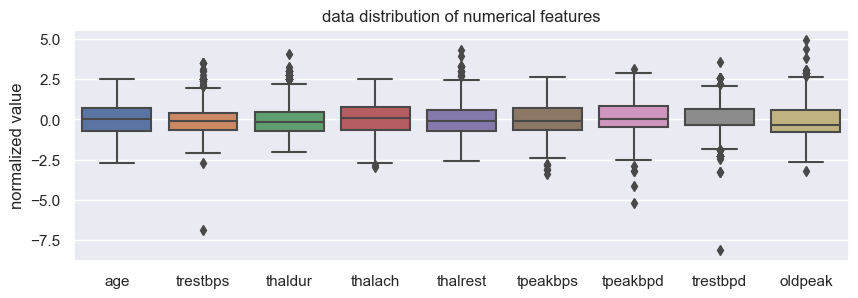
\includegraphics[width=\textwidth]{images/dataDistribution.png}
	\caption{data distribution of all numeric elements}
	\label{fig:dataDistribution}
\end{figure}
As shown in \cref{fig:dataDistribution}  normalised box plot of all numeric features were created to check for outliers. The features \textit{trestbps} and \textit{trestbpd} show extreme outliers with a value of 0. These are assumed to be incorrectly specified \texttt{NaN}s as stated in \cref{sec:dataUnderstanding} and are therefore replaced by \texttt{NaN}. All other outliers are not as extreme and come in groups. As the data contains sick persons, values diverging from the norm are expected. For these reasons it was decided to keep these outliers as they might be a strong indication of a heart disease.

After handling all errors in the dataset the categorical features \textit{cp, restecg, slope, ca, thal, restwm} were OneHotEncoded. All features were analysed regarding their pearson correlation, where only two pairs of features with a substantial amount of data ($<75\%$ \texttt{NaN}s) have a strong correlation ($>75\%$).  
These are asymptomatic chest pain $\leftrightarrow$ pain during exercise and \textit{rldv5} $\leftrightarrow$ \textit{rldv5e}. The first correlation seems plausible, as pain that only occurs under exercise is classified as asymptomatic. The features are still relevant, however, as the cases where there is no correlation are of particular interest. For \textit{rldv5} which denotes the height of the peak in the ECG during rest while \textit{rldv5e} is the same under exercise also the cases where there is no correlation are of special interest because this might be typical for people with a heart disease. In order to better understand the interrelationships two new features were computed. Both represent the difference between a peak and a resting measurement. Once for the ECG (\textit{rldv5\_diff}) and once for the blood pressure (\textit{thal\_diff}). 
Furthermore, the feature indicating whether a patient smokes was enhanced by using the number of cigarettes per day and the length of time a patient has been smoking to infer the boolean variable. Hereby, the number of \texttt{NaN}s was reduced from 74\% to 43\%. 

\subsection{Hyperparameter Tuning} \label{subsec:hyperparametertuning}
Additionally to the hyperparamter tuning of the estimators, which is described in \cref{sec:datamining}, the preprocessing steps were also optimised  by different hyperparameters.


Firstly, binning for the feature \textit{age} was added. Either 2, 5 bins or no binning at all are set as hyperparameters. The bins were encoded in an ordinal variable.

To impute the missing data a simple imputer was used. Missing values are replaced by the mean, median or mode of the feature. The KNN imputer was not used, because it is computationally much more expensive, while the iterative imputer is not used, as it is still experimental and therefore subject to change. Due to the high number of missing values and their uneven distribution across the features it was analysed how the number of imputed cells and number of features behave when columns with a certain amount of missing values are dropped. This is visualized in \cref{fig:percentageToBeDropped}.

\begin{figure}[h]
	\centering
	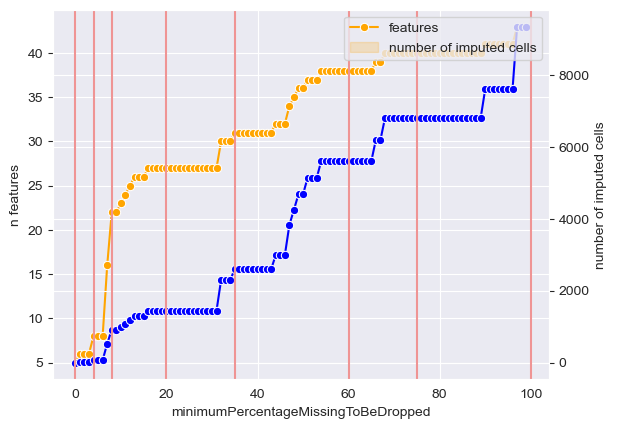
\includegraphics[width=\textwidth]{images/percentageToBeDropped.png}
	\caption{Number of features and values to be imputed by number of \texttt{NaN}s}
	\label{fig:percentageToBeDropped}
\end{figure}

It becomes apparent that there are certain steps where the number of features goes up a lot. To decide when a feature is included based on the number of missing values, the steps 0, 4, 8, 20, 35, 60, 75 and 100\% were set as hyperparameter. They are shown as vertical lines in the graph. 

To account for the different ranges of the features the MaxAbsScaler, MinMaxScaler, PowerTransformer, RobustScaler, Standardscaler and Normalizer are used. As the parameters of most scalers turn on or off core functionalities of the scaler, only tune the norm of the Normalizer was changed by hyperparameters with the norms l1, l2 and max.

To account for the slight imbalance of healthy and unhealthy patients oversampling and undersampling in the training data in comparison to no sampling was used. After this step the preprocessing is done. 


%The \textbf{MaxAbsScaler} scales the values of each feature by the maximum absolute value. Therefore, all values in [-1,1] can occur after scaling. \newline
%Using the \textbf{MinMaxScaler} results in values in [0,1] by shifting by the negative minimum and scaling by $maximum - minimum$\newline
%The values were normalized using the norms l1,l2 and max in the \textbf{Normalizer}. \newline
%The \textbf{PowerTransformer} alters the data to represent a gaußian like distribution. This is mostly used if heteroskedasticity occurs in the data. It was tried to fit the data to a standard normal distribution and without shifting and scaling by its mean and variance. \newline
%The \textbf{RobustScaler} was tried with and without scaling by the interquartile range and with and without shifting beforehand.\newline
%The \textbf{Standardscaler} was used with and without shifting by the mean and scaling by the standard deviation.\newline
%It was also tried, manly for comparison, to \textbf{passthrough} the values as they are.\newline